\documentclass[a4paper, 12pt, titlepage]{report}

%Taal: Nederlands ("Inhoudsopgave", "Hoofdstuk",...)
\usepackage{graphicx}
\usepackage{subcaption}
\usepackage{algorithmic}
\usepackage{amsmath, amssymb, textcomp, mathtools}
\usepackage{mcode}

%Hyperlinks
\usepackage{hyperref}

%Opmaak hyperlinks
\hypersetup{colorlinks=false,	urlcolor=cyan,pdfborder=0 0 0}

%Geen nummering bij secties en hoofdstukkden
\setcounter{secnumdepth}{-1} 

%geen indents
\setlength\parindent{0pt}

\usepackage{listings}
\lstset{
language=Matlab, % choose the language of the code
%basicstyle=10pt, % the size of the fonts that are used for the code
numbers=left, % where to put the line-numbers
numberstyle=\footnotesize, % the size of the fonts that are used for the line-numbers
stepnumber=1, % the step between two line-numbers. If it's 1 each line will be numbered
numbersep=5pt, % how far the line-numbers are from the code
%backgroundcolor=\color{grey}, % choose the background color. You must add \usepackage{color}
showspaces=false, % show spaces adding particular underscores
showstringspaces=false, % underline spaces within strings
showtabs=false, % show tabs within strings adding particular underscores
frame=single, % adds a frame around the code
%tabsize=2, % sets default tabsize to 2 spaces
%captionpos=b, % sets the caption-position to bottom
breaklines=true, % sets automatic line breaking
breakatwhitespace=false, % sets if automatic breaks should only happen at whitespace
escapeinside={\%*}{*)} % if you want to add a comment within your code
}


%"Figuur" in vet
\makeatletter
\renewcommand{\fnum@figure}{\small\textbf{\figurename~\thefigure}}
\makeatother

\usepackage[dutch]{babel}
\begin{document}

\title{\textbf{Numerieke Modellering en Benadering}}
\author{De Wolf Peter\\ Vekemans Wout}

\date{\today}
\begin{titlepage}
	\maketitle
	\thispagestyle{empty}
\end{titlepage}

\newpage
\tableofcontents

\listoffigures

\newpage
\section{Benaderen met veeltermen}
In dit practicum willen we eerst enkele functies benaderen met behulp van veeltermen door interpolatie. We gebruiken hierto nulpunten van orthogonale veeltermen als interpolatiepunten.
\subsection{Berekenen van nulpunten van orthogonale veeltermen}
\begin{lstlisting}
function x = poly_zeros(n, alpha, beta, lambda);

%maak diagonaalmatrix met de elementen van alpha
alphaMat = diag(alpha);

%maak matrices met mu en nu elementen op respectievelijk eerste boven- en
%onderdiagonaal
mu=zeros(n-1,1);
nu=zeros(n-1,1);
for i=1:n-1
    nu(i) = beta(i+1)/lambda(i+1);
    mu(i) = 1/lambda(i);
end
muMat = diag(mu,1);
nuMat = diag(nu,-1);

%maak matrix A
A= alphaMat+nuMat+muMat;

%bereken de eigenwaarden van A en dus de nulpunten van de veelterm
x=eig(A);
\end{lstlisting}
Deze functie berekent de nulpunten van de orthogonale veeltermen gebaseerd op de waarden $\alpha_k, \beta_k$, en $\lambda_k$ uit de recursiebetrekking voor orthogonale veeltermen \eqref{recursion}. Het doet dit door een tridiagonale matrix op te stellen met elementen afgeleid van de co\"efficienten uit die recursiebetrekking. De nulpunten van de veelterm zijn dan gelijk aan de eigenwaarden van die matrix.\\
\begin{subequations} \label{recursion}
\begin{align}
\phi_0(x) = \lambda_0\; ;\; \phi_1(x) = \lambda_1(x-\alpha_1)\phi_0(x))\\
\phi_k(x) = \lambda_k(x-\alpha_k)\phi_{k-1}(x))-\beta_k\phi_{k-2}(x)
\end{align}
\end{subequations}

\subsection{Evauleren van drietermsrecursiebetrekking}
\begin{lstlisting}
	function M = eval_recursion(x, n, alpha, beta, lambda)
	
	m = length(x);
	M=zeros(m,n);
	for i=1:m %itereer over rijen
	    M(i,1)=lambda(1);
	    M(i,2)=lambda(2)*(x(i)-alpha(1))*M(i,1);
	    for j=3:n %itereer over kolommen
	        M(i,j)=lambda(j)*(x(i)-alpha(j))*M(i,j-1)-beta(j)*M(i,j-2);
	    end
	end
\end{lstlisting}
Deze functie evalueert de drietermsrecursiebetrekking in de punten gegeven in de vector $x$. Als we deze methode toepassen op de 10 eerste Chebychev veeltermen krijgen we figuur \ref{chebychev}. Deze functie is eenvoudig toe te passen omdat Chebychev veeltermen duidelijk voldoen aan vergelijking \eqref{recursion}. Dit is makkelijk in te zien als men in de recursiebetrekking volgende waarden invult: $\lambda_0=1, \lambda_1=1$ en alle andere $\lambda_k$ gelijk aan 2. $\alpha_k$ is gelijk aan 0, en $\beta_k$ is 1. \\

\begin{figure}[htb]
	\centering
	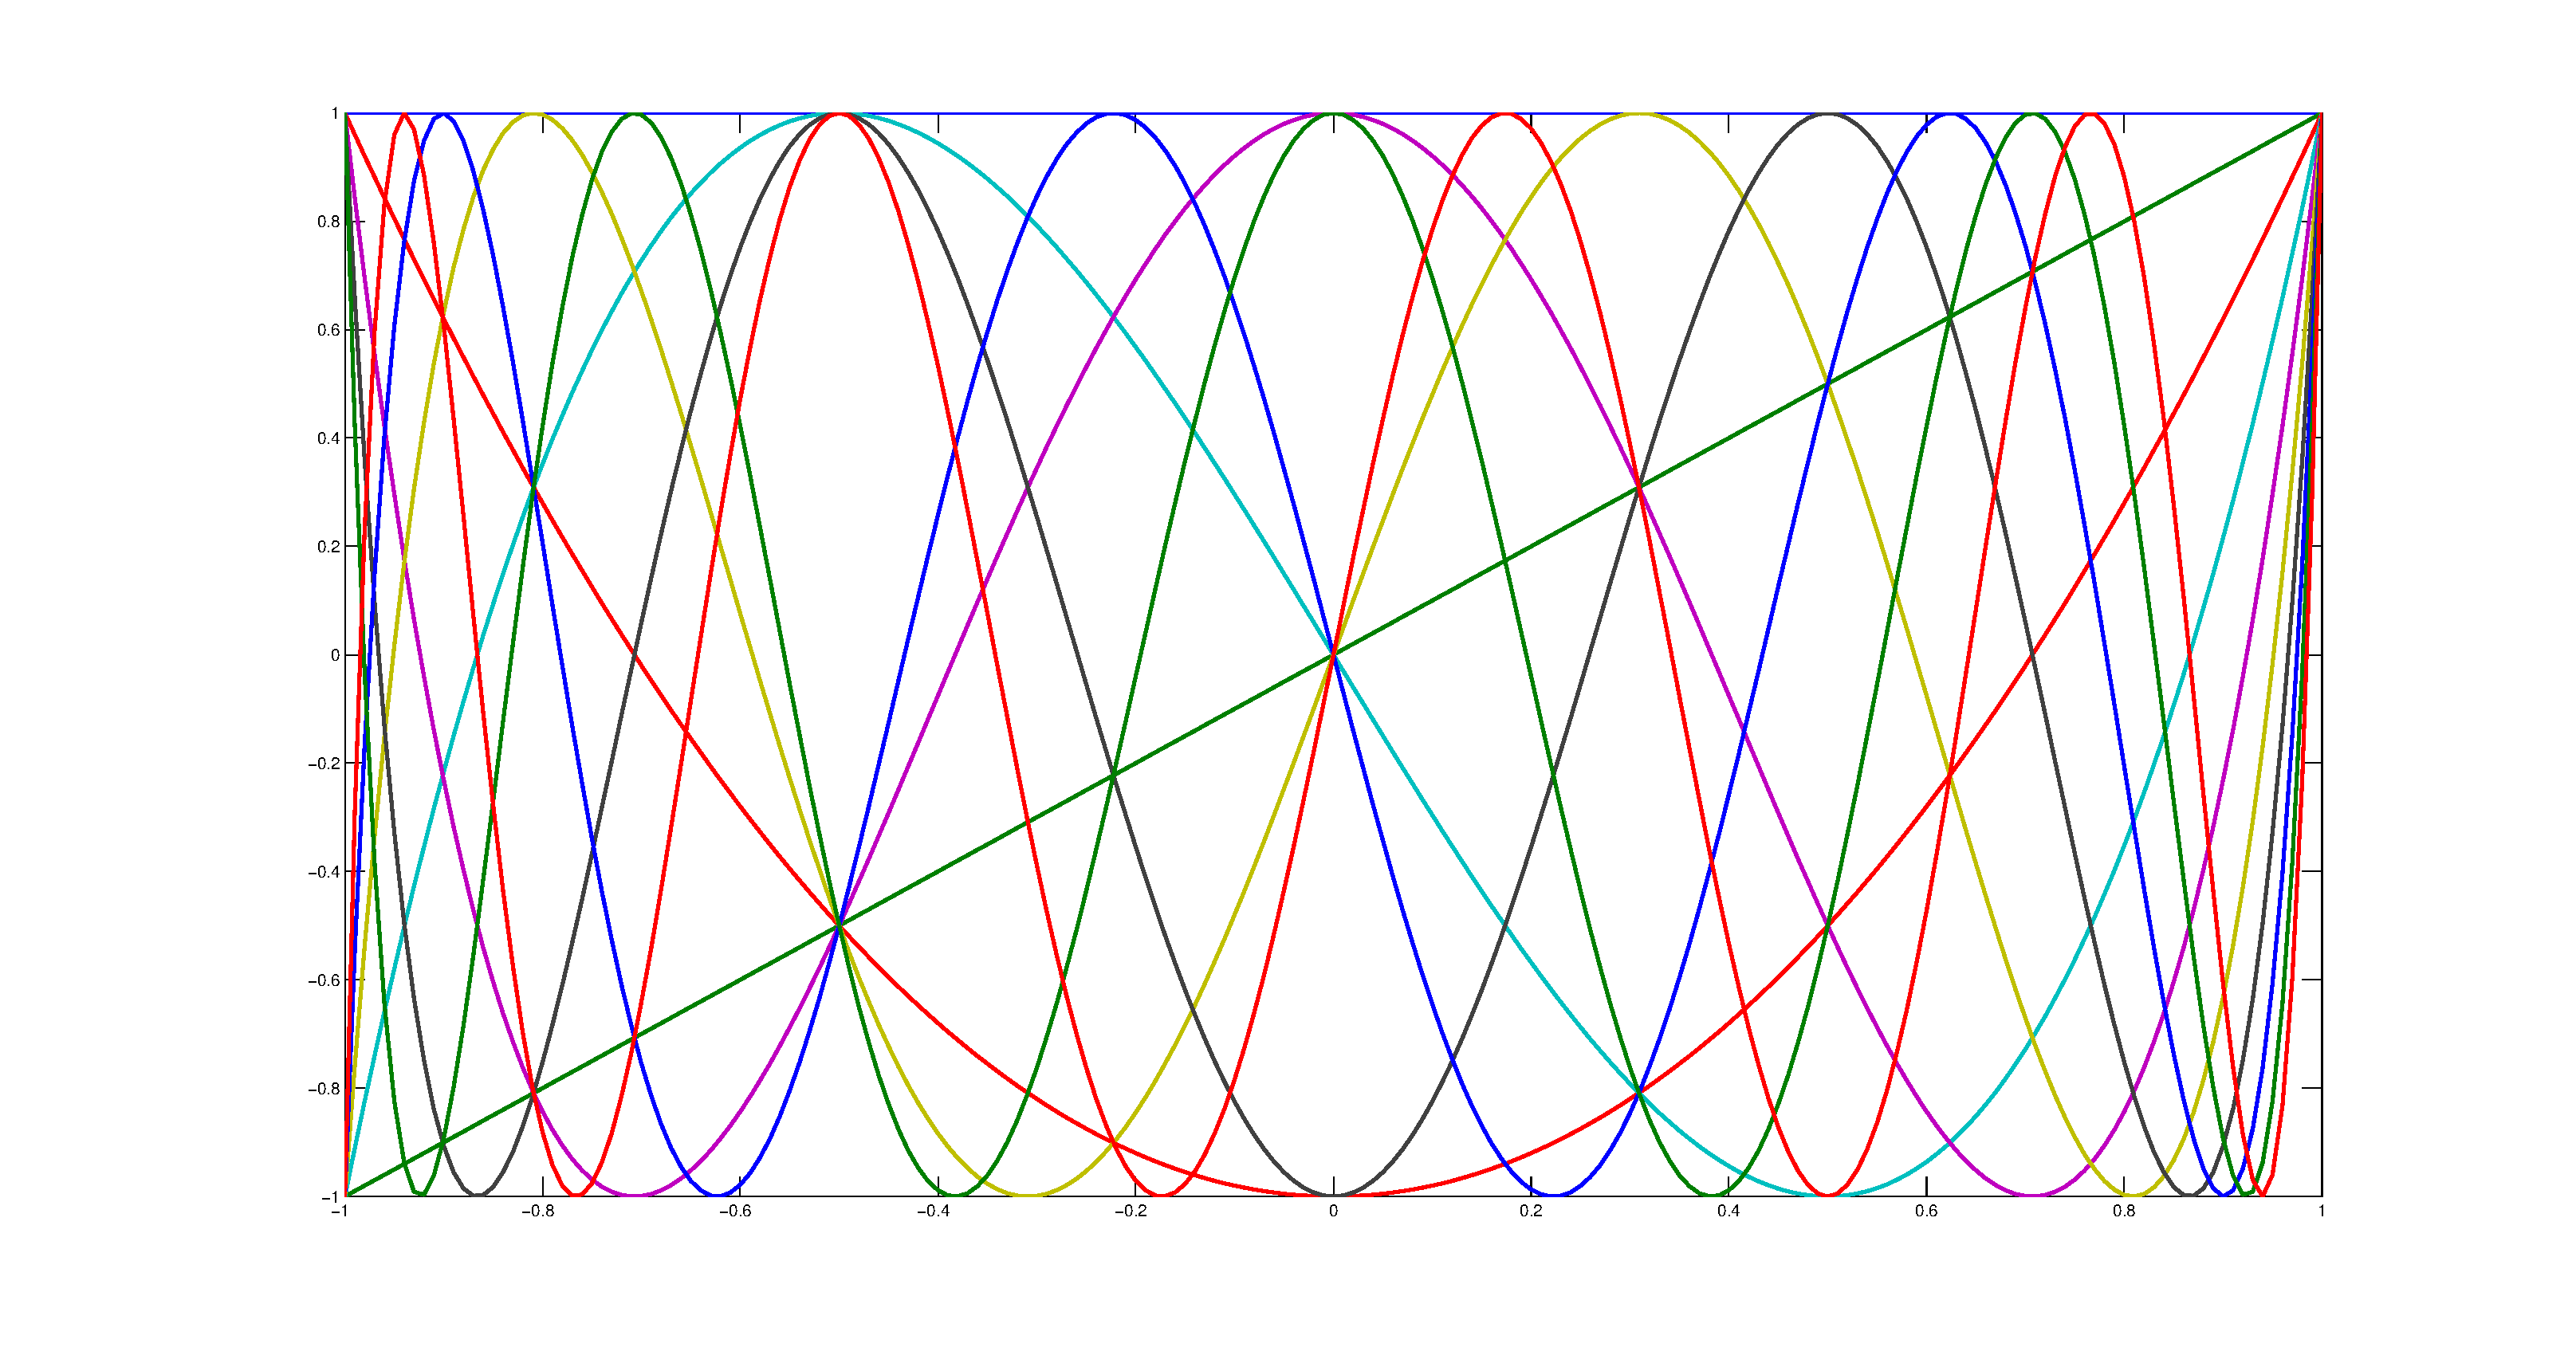
\includegraphics[width=\textwidth]{chebychev.eps}
	\caption{Evaluatie van eerste tien Cheybchev veeltermen op 200 punten in [-1,1]}
	\label{chebychev}
\end{figure}

\section{Berekenen van interpolerende veelterm}
\begin{lstlisting}
function y = interpolate(x, f, alpha, beta, lambda, t)

%maak M matrix
M=eval_recursion(x,length(alpha),alpha,beta,lambda);

%bereken de coefficienten van de interpolerende veelterm
c=M\f;

%bereken de waarden van de interpolerende veelterm in t
values=eval_recursion(t,length(alpha),alpha,beta,lambda);
res=values*c;
\end{lstlisting}
Als we met deze functie een interpolerende veelterm voor de functie $\cos(x)$ berekenen krijgen we figuur \ref{cosinus}. Op de grafiek zijn de interpolaties van graad 3, 5 en 10 weergegeven. De interpolatiefout voor die drie interpolerende functies zijn weergegeven op figuur \ref{abserrorcos}. We zien duidelijk dat een benadering van hogere graad nauwkeuriger is. Dit wordt ook ge\"illustreerd door figuur \ref{maxerrorcosinus}. Hierop is de maximale fout in functie van de graad van de interpolerende veelterm weergegeven. \\
\end{document}